\documentclass[twocolumn]{scndocument}
\usepackage{graphicx} % Required for inserting images
\usepackage{inputenc}

\graphicspath{ {images/} }

\usepackage{biblatex}
\addbibresource{bibliography.bib}

\usepackage{import}
\usepackage{scn} 

\usepackage{setspace}
\backgroundsetup{contents={}}
\pagestyle{plain}


\usepackage[russian]{babel} 

\begin{document}
 \setcounter{page}{168}
\begin{figure}[h]
    \centering
    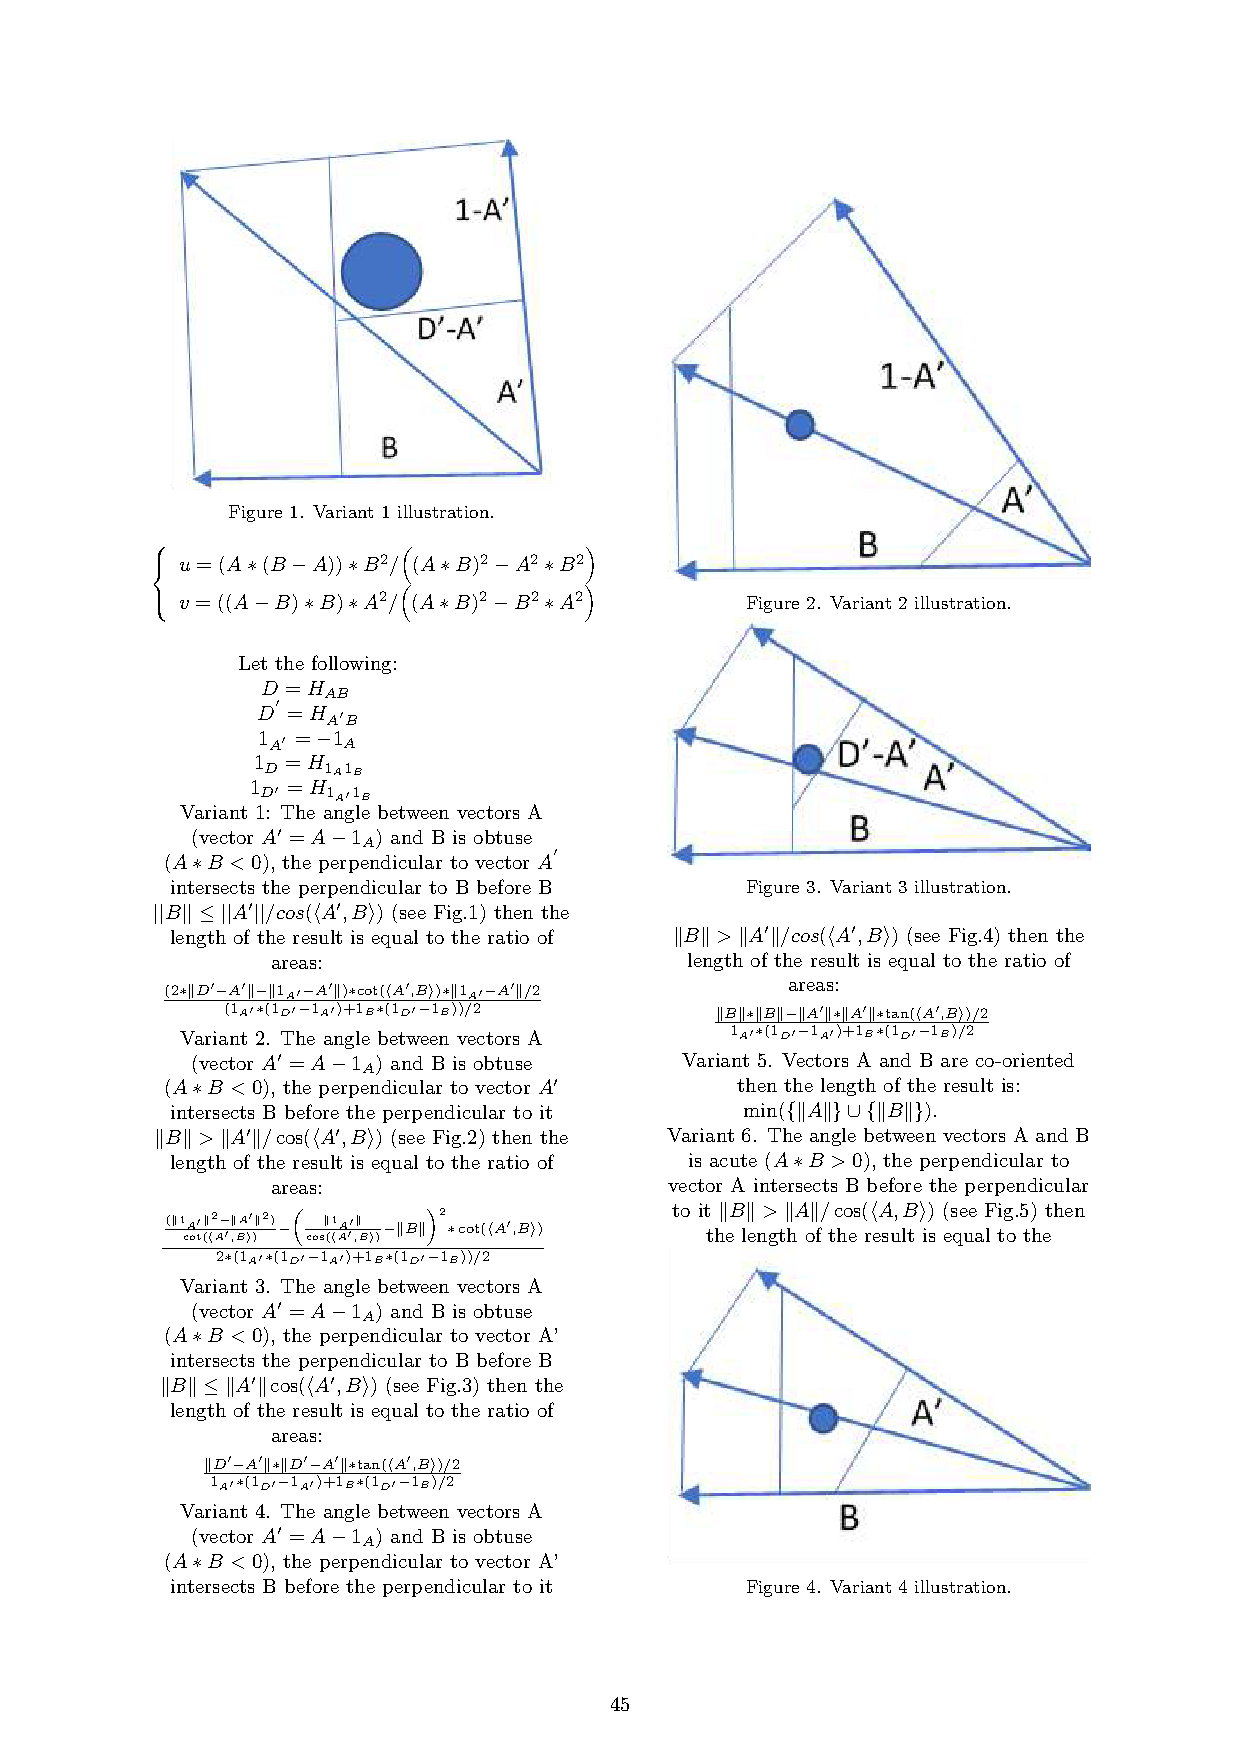
\includegraphics[width=\linewidth]{images/first.png} 
    \caption{Start page} 
    \label{Figure 1}
\end{figure}
$$y_j = F(\sum_{i}\omega_{ij} y_i - T_j ),$$
$$\gamma_{j} = y_{j} - t_{j} ,$$
$$\gamma_{i} = \sum_{i}\gamma{i}F^{'}(S_{j})\omega_{ji}$$ \begin{flushright} (2)\end{flushright}
$$\omega_{ij}(t + 1) = \omega_{ji}(t) - \alpha\gamma_{j}F^{'}(S_{j})y_i$$
$$T_{j}(t+1) = T_j(t) + \alpha\gamma_j F^{'} (S_j)$$
$$E = \frac{1}{2}\sum_{k=1}^{L} \sum_j (y_{j}^{k} - t_{j}^{k})^{2} $$

\par
To use the back propagation algorithm, we must select 
the E function, which must be minimized. It will be the
management error $e_{n}$ at the time $t = nT_{0}$ - get $E_{n} = \frac{1}{2}e^{2}_{n}$
. To accumulate errors, we store the data we have
previously obtained — $E_{n-p}$, ...$E_{n-2}$, $E_{n-1}$, $E_{n}$, where
p determines the number of previously saved images used
for network learning (2).
\vspace{2 mm} 
\\ \MakeUppercase{\romannumeral 5}. Examples of system operation with natural language
information display 
\vspace{2 mm}
\par
For information to be clear and understandable to the
reader, it must be presented in a consistent manner. The
recipe authoring system interface allows the structure of
domains and ontologies to be expressed in natural language. This process of converting an internal knowledge
representation to an external knowledge representation
is performed by a graphical interface component. On
the main page general information (in 4 languages) is
displayed, Figure 1. \ref{Figure 1}. \par
Fig. 6 shows resulting ontologies for standards (ISA88, SCg).
\vspace{2 mm}
\begin{center}
 \MakeUppercase{\romannumeral 6}. Integration of third-party solutions with a knowledge base
 \end{center}
\par A standard system built on the basis of OSTIS Technology can be easily integrated with other systems in
the workplace. To integrate ISA-88, ISA-95 and ISA5.1 standards system with other systems running on JSC
"Savushkin Product", a web-oriented approach is used -
\newpage
\begin{figure}[h]
    \centering
    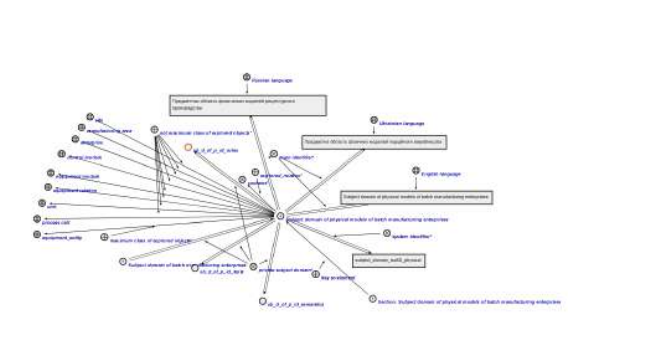
\includegraphics[width=\linewidth]{images/second.png}
    \label{Figure 7} 
    \caption{Ontologies for standard ISA-88}
\end{figure}
\begin{figure}[h]
    \centering
    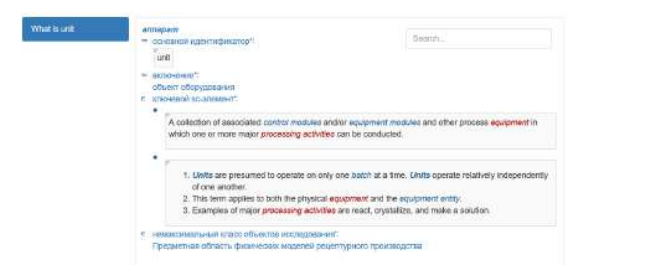
\includegraphics[width=\linewidth]{images/second&third.png}
    \caption{Unit}
    \label{Figure 8}
\end{figure}

the ostis-system server is accessed with the use of the
following queries:
\textit{$$h t t p : / / i n d u s t r y . o s t i s . n e t ? s y s _ i d = u n i t$$}
where "sys id=unit" defines a term (the name of an
entity) whose value we want to find out (in this example,
in fact, the answer to the question "What is a "unit"?).
This approach makes it relatively easy to add support of
the knowledge base for current control systems projects,
for this it is enough to indicate the names corresponding
to the entities in the knowledge base within the control
system. The answer is shown on Fig. 7 \ref{Figure 7}.

Thus, an interactive intelligent help system for control
systems projects is implemented, allowing employees to
simultaneously work with the control system and ask
questions to the system directly during the work.

Another example is the integrated help subsystem
within corporate Add-In \textbf{EasyEPLANner} [17] for CAD
EPLAN. It helps to describe technological objects (Tank,
Boiler, etc.), operations, etc. according to the ISA-88
standard. Fig. 8 shows UML-model of EasyEPLANner
objects to be described in OSTIS. The \textbf{PID controller}
is at the lower level — the control module (highlighted
by the green). It can be replaced by the development
\textbf{neuro-PID controller}.

 \begin{center}
\MakeUppercase{\romannumeral 7}. Use in control systems
\end{center}

It is very important to correct and fast react on
different events during process control, especially on
critical accidents. But when we have complex distributed
system it is rather complicated and in normal way require
help of the human operator. It may leads to variety of
\newpage

\begin{figure}[h]
    \centering
    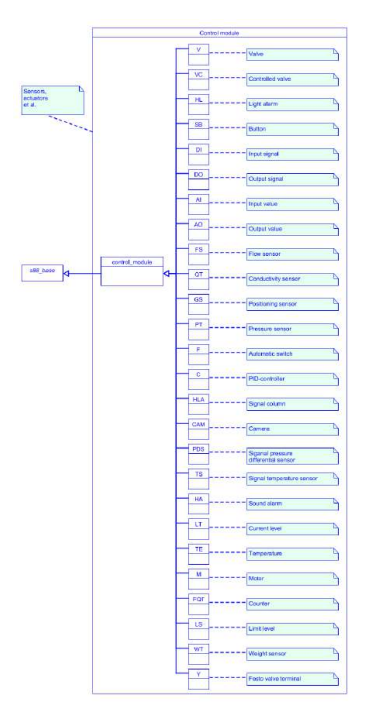
\includegraphics[width=\linewidth]{images/third.png}
    \caption{\textbf{EasyEPLANner} objects}
    \label{Figure 9}
\end{figure}
problems. So usage OSTIS-based system can helps to
solve as described on Fig. 9 \ref{Figure 9}. Project \#2 has a valve failure
but the project does not know what to do. Then it makes a
request to the OSTIS server, which already knows which
projects also use this line (with this valve). The OSTIS
server polls the rest of the projects (projects \#1 and \#2).
Each project has information about which operations are
currently active and gives an answer on what to do —
pause the operation, do nothing, etc. After that OSTISserver sends back to project \#2 answer with result actions
to be used. These are going in automatic way — no need
of human operator.
\begin{center}
  \MakeUppercase{\romannumeral 8}. Future development
\end{center}


Current project issues can be found on GitHub ( [18],
[19] and [20]). Main problems to be solved are:
\newpage

\begin{figure}[h]
    \centering
    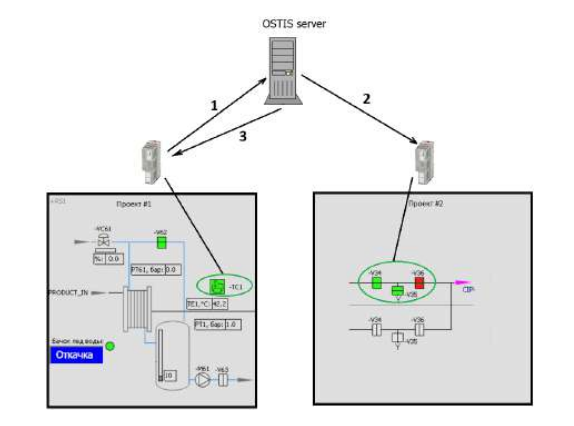
\includegraphics[width=\linewidth]{images/fourth.png} 
    \caption{OSTIS in control systems}
    \label{рис 10}
\end{figure}


\begin{itemize}
\item  Improving system performance and especially accelerating system response time to user requests.
It is connect with productivity and overall user
satisfaction.

\item Continuous updating and refactoring ontological
models (further formalization of missing concepts,
fix typos and etc.);

\item  Enhancing PFC-visualization - not only displaying,
but also editing diagrams. Adding rich navigating
between PFC-diagram and according text representation;

\item  Further formulation of questions (typical) to the
system from the user and their formalization at the
level of the existing knowledge base;

\item Adding more description of parts of real control
projects based on the existing knowledge base.
\end{itemize}

The implementation of answers to complex questions
is necessary to make easier the work of not only process
operators, but also maintenance personnel — instrumentation engineers, mechanics, electricians, etc. Therefore,
it is planned to implement the system’s answer to the
question of the following type — in what operations
of which objects this actuator is used (for example,
valve \textbf{"T1V1"}). This question is very important when a
device failure occurs and it is necessary to determine the
criticality of this situation. For analysis, it is necessary
to compare the time of the accident and the history of
operations. Since, for example, an accident of the mixproof valve during the line washing operation and the
active product dosing along the other line, should lead
to a stop of these operations and stop the preparation of
the batch in the corresponding unit. The operator must
report this to the appropriate maintenance specialist to
fix it. After the fault has been eliminated, the operator
continues to perform operations. This is the correct
events order, which is very important to avoid mixing of
detergent and product. If the device malfunction occurred
\newpage

within the line, which is now inactive, then this situation
has a low priority, does not lead to a stop in operations
and can be eliminated later if the service personnel have
free time.

\singlespacing
\begin{center}
\MakeUppercase{\romannumeral 9}. Conclusion  
\end{center}

The paper considers an technique to automating the
process of creating, developing and making use of standards primarily based on OSTIS Technology. Using the
instance of the ISA-88, ISA-95 and ISA-5.1 standards
used on the Savushkin Product enterprise, the structure
of the knowledge base, the features of the problem solver
and the user interface of the support system for these
processes are considered. It is proven that the developed
system can be easily integrated with other enterprise
systems, being the basis for building an information
service system for employees in the context of Industry
4.0. The approach proposed in the work allows us to
provide not only the ability to automate the processes
of creation, agreeing and development of standards, but
also allows us to significantly increase the efficiency of
the processes of applying the standard, both in manual
and automatic way.

\singlespacing
\begin{center}
    Acknowledgment
\end{center}

Author would like to thank to the research teams of
the Departments of intelligent information technologies
of the Belarusian State University of Informatics and Radioelectronics and the Brest State Technical University.

\singlespacing
\begin{center}
    References
\end{center}
\begin{enumerate}[label=\textbf{[\arabic*]}]
  \printbibliography
\item \footnotesize {N. Lutska, O. Pupena, A. Shyshak, V. Taberko, D.e Ivaniuk, M. O. Nikita Zotov, and L. Vlasenko, “Ontological model of digital twin
in manufacturing,” in \underline{Open semantic technolo} \\ \underline{gies for intelligent systems}, ser. 5, V. Golenkov, Ed. BSUIR, Minsk, 2022, p.
310–335.
\item  V. V. Taberko, D. S. Ivaniuk, D. V. Shunkevich, and O. N. Pupena,
“Principles for enhancing the development and use of standards
within Industry 4.0,” in \underline{Open semantic techno} \\ \underline{logies for intelligent systems}, ser. 4, V. Golenkov, Ed. BSU \\ IR, Minsk, 2020, pp. 167–
174.
\item V. A. Golovko, A. A. Kroshchanka, V. V. Golenkov, V. P.
Ivashenko, M. V. Kovalev, V. V. Taberko, and D. S. Ivaniuk,
“Integration of artificial neural networks and knowledge bases,”
2018.
\item S. Gil, G. D. Zapata-Madrigal, and G. L. Giraldo-Gómez, “An ontological model to integrate and assist virtualization of automation
systems for industry 4.0,” \underline{Smart and Sustain} \\ 
\underline{able Manufacturing Systems}, vol. 5, p. 10, 09 2021.
\item  V. R. Sampath Kumar, A. Khamis, S. Fiorini, J. L. Carbonera, A. Olivares Alarcos, M. Habib, P. Goncalves, H. Li, and
J. I. Olszewska, “Ontologies for industry 4.0,” \underline{The Knowledge
En} \\ \underline{gineering Review}, vol. 34, p. e17, 2019.
\item  V. Golenkov, N. Gulyakina, I. Davydenko, and
D. Shunkevich, “Semanticheskie tekhnologii proektirovaniya
intellektual’nyh sistem i semanticheskie associativnye
komp’yutery [Semantic technologies of intelligent
systems design and semantic associative computers],”
\underline{Open semantic technologies for in-} \\ \underline{telligent systems}, pp. 42–
50, 2019.
\item  “Digital Twins for Industrial Applications, an Industrial Internet
Consortium White Paper” $https://www.iiconsor$ \\ $tium.org/pdf/IIC_
Digital\_Twins\_Industrial\_Ap\\ps\_White\_Paper\_2020-02-18.pdf$,
2018.

\item  M. Sverko, T. G. Grbac, and M. Mikuc, “Scada systems with
focus on continuous manufacturing and steel industry: A survey
on architectures, standards, challenges and industry 5.0,” \underline{IEEE
Access}, vol. 10, pp. 109 395–109 430, 2022.
\item  P. Serenkov, V. Solomaho, V. Nifagin, and A. Minova, “Koncepcija infrastruktury standartizacii kak bazy znanij na osnove
ontologij [the concept of a standardization infrastructure as
an ontology-based knowledge base],” \underline{Novos} \\ \underline{ti. Standartizacija i sertifikacija.[News. Standardization and} \\ \underline{ certification.]}, vol. 1,
no. 5, pp. 25–29, 2004.
\item  V. Uglev, “Aktualizacija soderzhanija standartov proektirovanija
slozhnyh tehnicheskih ob’ektov: ontologicheskij podhod [updating the content of design standards for complex technical objects:
ontologic approach],” \underline{Ontologija proektirovanija.} \\ \underline{[Ontology of
designing]}, vol. 1, no. 1, pp. 80–86, 2012.
\item  C. Dombayci, J. Farreres, H. Rodríguez, A. Espuña, and
M. Graells, “Improving automation standards via semantic modelling: Application to ISA88,” \underline{ISA Transactions}, vol. 67, 01 2017.
\item  M. Vegetti and G. Henning, “Isa-88 formalization. a step towards
its integration with the isa-95 standard,” in \underline{6th Workshop} \\ \underline{on
Formal Ontologies me} \\ \underline{et Industry}, vol. 1333, 02 2015.
\item  “ISA-88 standard,” https://www.isa.org/standards-andpublica- \\tions/isa-standards/isa-standards-committees/isa88/,
(accessed 2022, October).
\item  “ISA-95 standard,” https://www.isa.org/standards-andpublica- \\ tions/isa-standards/isa-standards-commi \\ ttees/isa95/,
(accessed 2022, October).
\item  A. A. Uskov and A. V. Kuz’min, \underline{Intellektual’nye tek} \\ \underline{hnologii
upravleniya. Iskusstvennye nejronnye seti} \\ \underline{i nechetkaya logika}.
Goryachaya liniya - Telekom, 2004.
\item  D. S. Ivaniuk, “Neuro-pid controller for a pasteurizer,” in
\underline{XV International PhD Workshop OWD}, 2013.
\item  “EasyEPLANner project on GitHub,” Available at: https://github.
com/savushkin-r-d/EasyEPLANner/, (accessed 2022, Jun).
\item  “EasyServer-4.0 project on GitHub,” Available at: https://github.
com/savushkin-r-d/EasyServer-4.0, (accessed 2024, Feb).
\item “s88-ostis project on GitHub,” Available at: https:// \\ github.com/
savushkin-r-d/s88-ostis, (accessed 2024, Feb).
\item  “isa-5.1-ostis project on GitHub,” Available at: https://github.com/
savushkin-r-d/isa-5.1-ostis, (accessed 2024, Feb).}
\end{enumerate}  
\begin{center}

\textbf{НЕЙРО-СЕМАНТИЧЕСКОЕ} \par
\textbf{УПРАВЛЕНИЕ В} \par
\textbf{ПРОМЫШЛЕННОСТИ} \par

\large{Иванюк Д. С.}   
\end{center}
\footnotesize{
\par В работе рассмотрен онтологический подход к пониманию,
интеграции и развитию современных подходов к управлению
(нейроуправление, семантические технологии, современные
международные стандарты) с использованием Технологии
OSTIS. Уточнены формальные трактовки основных понятий,
используемых в стандартах, что позволяет упростить опи-
сание реальных задач. Также описаны варианты интеграции
базы знаний в используемые программные средства разработ-
ки и сценарии её использования непосредственно в системах
управления.} 
\begin{flushright}
Received 01.04.2024
\end{flushright}
\end{document}
